\clearpage %&latex
\documentclass[a4paper]{article}

\frenchspacing

\usepackage[cp1250]{inputenc}
\usepackage[czech]{babel}

\usepackage{a4wide}
\usepackage{amsmath, amsthm, amssymb, amsfonts}
\usepackage[mathcal]{eucal}
\usepackage{graphicx}
\usepackage{url}
\usepackage{color}
\usepackage{wrapfig}
\usepackage{capt-of}
\usepackage{float}



% sirka a vyska textu nastavena jako papir, vsechny okraje vynulovany a pridano 20pt na kazdou stranu
% horizontalni rozmery
\setlength{\textwidth}{\paperwidth}
\addtolength{\textwidth}{-40pt}
\addtolength{\hoffset}{-1in}
\addtolength{\hoffset}{20pt}
\setlength{\oddsidemargin}{0in}
\setlength{\marginparsep}{0in}
% vertikalni rozmery
\setlength{\textheight}{\paperheight}
\addtolength{\textheight}{-60pt}
\addtolength{\voffset}{-1in}
\addtolength{\voffset}{20pt}
\setlength{\topmargin}{0in}
\setlength{\headheight}{0in}
\setlength{\headsep}{0in}


%Obrazek na miste
%pouziti
%%\obrazeknahore{adresa}{popisek}{label}
\long\def\obrazeknahore#1#2#3 {

\begin{figure}[t]
    \centering
    \includegraphics[width=0.8\textwidth]{#1}
    
    \caption{#2}
    \label{#3}
    
\end{figure}

}


%==========================================
%PEKELNA MAKRA NA ZAROVNANI OBRAZKU DOPRAVA

\makeatletter


%tohle je makro, ktere mi dovoluje obtekani i u kratkych environmentu
%ABSOLUTNE nechapu, jak to funguje, ale funguje to
%viz http://tex.stackexchange.com/questions/26078/ 
\def\odrovnej{\@@par
\ifnum\@@parshape=\z@ \let\WF@pspars\@empty \fi % reset `parshape'
\global\advance\c@WF@wrappedlines-\prevgraf \prevgraf\z@
\ifnum\c@WF@wrappedlines<\tw@ \WF@finale \fi}

\makeatother



%---
%makro, co da obrazek doprava a ostatni text ho obteka
%(bez toho predchazejiciho makra to ale poradne nebeha)
%pouziti:
%\obrazekvpravo{adresa}{popisek}{label}{procento sirky}
\long\def\obrazekvpravo#1#2#3#4{

\setlength\intextsep{-20pt}

    \begin{wrapfigure}{r}{#4\textwidth}
      \begin{center}
          \vspace{-10pt}
          
        \includegraphics[width=#4\textwidth]{#1}
        \vspace{-10pt}
        
      \end{center}
      
      \caption{#2}
      \label{#3}
      
      
    \end{wrapfigure}

\setlength\intextsep{0pt}

    
}




%---
%makro pro pripady, kdy wrapfigure neco mrsi
%je to docela pekelne
%je nutne mu dat jak text vpravo, tak text vlevo
%a nevim, jestli bude 100% fungovat, ale doufam, ze jo

%pouziti:
%\obrazekvpravominipage{adresa}{popisek}{label}{procento sirky}{1 - procento sirky}{text vlevo}
\long\def\obrazekvpravominipage#1#2#3#4#5#6{

\noindent\begin{minipage}{#5\linewidth}
\vspace{0pt}
#6
\end{minipage}
\hspace{0.5cm}
\noindent\begin{minipage}{#4\linewidth}
\vspace{0pt}
\centering
\includegraphics[width=0.9\textwidth]{#1}
\captionof{figure}{#2}
\label{#3}
\end{minipage}

}

%KONEC PEKELNYCH MAKER
%=====================

% makra pro poznamku u vyrokove a predikatove logiky
\def\vl{ -- ve v�rokov� logice}
\def\pl{ -- v predik�tov� logice}


%Vacsina prostredi je dvojjazicne. V pripade, ze znenie napr pozorovania je pisane po slovensky, malo by byt po slovensky aj oznacenie.

\newenvironment{pozadavky}{\pagebreak[2]\noindent\textbf{Po�adavky}\par\noindent\leftskip 10pt}{\odrovnej\par\bigskip}
\newenvironment{poziadavky}{\pagebreak[2]\noindent\textbf{Po�iadavky}\par\noindent\leftskip 10pt}{\odrovnej\par\bigskip}


\newenvironment{definiceSkull}{\pagebreak[2]\noindent\textbf{$\bigstar$ Definice}\par\noindent\leftskip 10pt}{\odrovnej\par\bigskip}
\newenvironment{definiceNSkull}[1]{\pagebreak[2]\noindent\textbf{$\bigstar$ Definice~}\emph{(#1)}\par\noindent\leftskip 10pt}{\odrovnej\par\bigskip}

\newenvironment{definice}{\pagebreak[2]\noindent\textbf{Definice}\par\noindent\leftskip 10pt}{\odrovnej\par\bigskip}
\newenvironment{definiceN}[1]{\pagebreak[2]\noindent\textbf{Definice~}\emph{(#1)}\par\noindent\leftskip 10pt}{\odrovnej\par\bigskip}
\newenvironment{definicia}{\pagebreak[2]\noindent\textbf{Defin�cia}\par \noindent\leftskip 10pt}{\odrovnej\par\bigskip}
\newenvironment{definiciaN}[1]{\pagebreak[2]\noindent\textbf{Defin�cia~}\emph{(#1)}\par\noindent\leftskip 10pt}{\odrovnej\par\bigskip}

\newenvironment{vetaSkull}{\pagebreak[2]\noindent\textbf{$\bigstar$ V�ta}\par\noindent\leftskip 10pt}{\odrovnej\par\bigskip}
\newenvironment{vetaNSkull}[1]{\pagebreak[2]\noindent\textbf{$\bigstar$ V�ta~}\emph{(#1)}\par\noindent\leftskip 10pt}{\odrovnej\par\bigskip}

\newenvironment{pozorovani}{\pagebreak[2]\noindent\textbf{Pozorov�n�}\par\noindent\leftskip 10pt}{\odrovnej\par\bigskip}
\newenvironment{pozorovanie}{\pagebreak[2]\noindent\textbf{Pozorovanie}\par\noindent\leftskip 10pt}{\odrovnej\par\bigskip}
\newenvironment{poznamka}{\pagebreak[2]\noindent\textbf{Pozn�mka}\par\noindent\leftskip 10pt}{\odrovnej\par\bigskip}
\newenvironment{poznamkaN}[1]{\pagebreak[2]\noindent\textbf{Pozn�mka~}\emph{(#1)}\par\noindent\leftskip 10pt}{\odrovnej\par\bigskip}
\newenvironment{lemma}{\pagebreak[2]\noindent\textbf{Lemma}\par\noindent\leftskip 10pt}{\odrovnej\par\bigskip}
\newenvironment{lemmaN}[1]{\pagebreak[2]\noindent\textbf{Lemma~}\emph{(#1)}\par\noindent\leftskip 10pt}{\odrovnej\par\bigskip}
\newenvironment{veta}{\pagebreak[2]\noindent\textbf{V�ta}\par\noindent\leftskip 10pt}{\odrovnej\par\bigskip}
\newenvironment{vetaN}[1]{\pagebreak[2]\noindent\textbf{V�ta~}\emph{(#1)}\par\noindent\leftskip 10pt}{\odrovnej\par\bigskip}
\newenvironment{vetaSK}{\pagebreak[2]\noindent\textbf{Veta}\par\noindent\leftskip 10pt}{\odrovnej\par\bigskip}
\newenvironment{vetaSKN}[1]{\pagebreak[2]\noindent\textbf{Veta~}\emph{(#1)}\par\noindent\leftskip 10pt}{\odrovnej\par\bigskip}

\newenvironment{dusledek}{\pagebreak[2]\noindent\textbf{D�sledek}\par\noindent\leftskip 10pt}{\odrovnej\par\bigskip}
\newenvironment{dosledok}{\pagebreak[2]\noindent\textbf{D�sledok}\par\noindent\leftskip 10pt}{\odrovnej\par\bigskip}

\newenvironment{dokaz}{\pagebreak[2]\noindent\leftskip 10pt\textbf{D�kaz}\par\noindent\leftskip 10pt}{\odrovnej\par\bigskip}
\newenvironment{dukaz}{\pagebreak[2]\noindent\leftskip 10pt\textbf{D�kaz}\par\noindent\leftskip 10pt}{\odrovnej\par\bigskip}

\newenvironment{ideadukazu}{\pagebreak[2]\noindent\leftskip 10pt\textbf{Idea d�kazu}\par\noindent\leftskip 10pt}{\odrovnej\par\bigskip}


\newenvironment{priklad}{\pagebreak[2]\noindent\textbf{P��klad}\par\noindent\leftskip 10pt}{\odrovnej\par\bigskip}
\newenvironment{prikladN}[1]{\pagebreak[2]\noindent\textbf{P��klad~}\emph{(#1)}\par\noindent\leftskip 10pt}{\odrovnej\par\bigskip}

\newenvironment{prikladSK}{\pagebreak[2]\noindent\textbf{Pr�klad}\par\noindent\leftskip 10pt}{\odrovnej\par\bigskip}
\newenvironment{priklady}{\pagebreak[2]\noindent\textbf{P��klady}\par\noindent\leftskip 10pt}{\odrovnej\par\bigskip}
\newenvironment{prikladySK}{\pagebreak[2]\noindent\textbf{Pr�klady}\par\noindent\leftskip 10pt}{\odrovnej\par\bigskip}

\newenvironment{algoritmusN}[1]{\pagebreak[2]\noindent\textbf{Algoritmus~}\emph{(#1)}\par\noindent\leftskip 10pt}{\odrovnej\par\bigskip}
%obecne prostredie, ktore ma vyuzitie pri specialnych odstavcoch ako (uloha, algoritmus...) aby nevzniklo dalsich x prostredi
\newenvironment{obecne}[1]{\pagebreak[2]\noindent\textbf{#1}\par\noindent\leftskip 10pt}{\odrovnej\par\bigskip}

\newenvironment{report}{\pagebreak[2]\noindent\textbf{Report}\em\par\noindent\leftskip 10pt}{\par\bigskip}

%\newenvironment{reportN}[1]{\pagebreak[2]\noindent\textbf{Report~}\emph{(#1)}\emph\par\noindent\leftskip 10pt}{\odrovnej\par\bigskip}
\newenvironment{reportN}[1]{\pagebreak[2]\noindent\textbf{Report~}\emph{(#1)}\em\par\noindent\leftskip 10pt}{\odrovnej\par\bigskip}

\newenvironment{penumerate}{
\begin{enumerate}
  \setlength{\itemsep}{1pt}
  \setlength{\parskip}{0pt}
  \setlength{\parsep}{0pt}
  %\setlength{\topsep}{200pt}
  \setlength{\partopsep}{200pt}
}{\end{enumerate}}

\def\pismenka{\numberedlistdepth=2} %pouzit, ked clovek chce opismenkovany zoznam...

\newenvironment{pitemize}{
\begin{itemize}
  \setlength{\itemsep}{1pt}
  \setlength{\parskip}{0pt}
  \setlength{\parsep}{0pt}
}{\end{itemize}}

%\definecolor{gris}{gray}{0.95}
\newcommand{\ramcek}[2]{\begin{center}\fcolorbox{white}{gris}{\parbox{#1}{#2}}\end{center}\par}
 \clearpage
\title{\LARGE U�ebn� texty k st�tn� bakal��sk� zkou�ce \\ Programov�n� \\ Z�klady teoretick� informatiky}
\begin{document}
\maketitle
\newpage
\setcounter{section}{0}
\section{Z�klady teoretick� informatiky}
\begin{e}{Po�adavky}{0}{0}
\begin{pitemize}
\item Logika - jazyk, formule, s�mantika, tautologie
\item Rozhodnutelnost, splnitelnost, pravdivost, dokazatelnost
\item Norm�ln� tvary v�rokov�ch formul�, prenexn� tvary formul� predik�tov� logiky
\item Automaty - Chomsk�ho hierarchie, t��dy automat� a gramatik, determinismus a nedeterminismus.
\end{pitemize}
\end{e}
\def\c#1{\mathcal{#1}}


\subsection{Jazyk, formule, s�mantika, tautologie}

\begin{obecne}{logika prvn�ho ��du}
V logice pracujeme s formulemi a termy, co� jsou slova (�et�zce znak� dan� abecedy) form�ln�ho jazyka. Jazyk prvn�ho ��du m��e zahrnovat:
\begin{pitemize}
    \item neomezen� mnoho symbol� pro prom�nn� $x_1,x_2,\dots $
    \item symboly pro logick� spojky ($\neg,\vee,\&,\rightarrow,\leftrightarrow$)
    \item symboly pro kvantifik�tory ($\forall$ obecn�, $\exists$ existen�n�)
    \item funk�n� symboly $f_1,f_2\dots $ s aritou $n \geq 0$ (nap�. $+, -, 1, *$)
    \item predik�tov� symboly $p_1,p_2\dots $ s aritou $n \geq 1$ (nap�. $\geq, =, \approx, \in, \subset $)
    \item m��e (ale nemus�) obsahovat bin�rn� predik�t \uv{$=$}, kter� pak se pak ale mus� chovat jako rovnost, tj. spl�ovat ur�it� axiomy.
\end{pitemize}
Prom�nn�, logick� spojky, kvantifik�tory a \uv{$=$} jsou \emph{logick� symboly}, ostatn� symboly se naz�vaj� \emph{speci�ln�}, jeliko� ur�uj� specifika jazyka a t�m vymezuj� oblast, kterou jazyk popisuje. V�rokov� a predik�tov� logika se �ad� mezi logiky prvn�ho ��du. Ty pracuj� jen s jazyky prvn�ho ��du, kter� maj� pouze jeden typ prom�nn�ch (pro prvky zvan� \emph{individua}). Jazyky vy���ch ��d� maj� krom� prom�nn�ch pro individua tak� dal�� typy prom�nn�ch (pro p�irozen� ��sla, funkce, relace, mno�iny a dal�� typy objekt�).

Ka�d� \emph{form�ln� syst�m} logiky prvn�ho ��du obsahuje:
\begin{pitemize}
    \item jazyk
    \item axiomy
    \item odvozovac� pravidla (pomoc� nich� tvo��me d�kazy a odvozujeme v�ty).
\end{pitemize}
Ze symbol� jazyka tvo��me dva druhy slov:
\begin{pitemize}
    \item \emph{termy} popisuj� individua (objekty) vznikl� z uveden�ch operac�
    \item \emph{formule} vyjad�uj� tvrzen� o objektech.
\end{pitemize}
\end{obecne}

\begin{definiceN}{jazyk v�rokov� logiky}
Jazyk $L_P$ v�rokov� logiky nad mno�inou $P$ obsahuje prvky mno�iny $P$ zvan� \emph{prvotn� formule} nebo \emph{v�rokov� prom�nn�} (typicky jde o slova n�jak�ho form�ln�ho jazyka nap�. $x, y, ABC, nula$), symboly pro \emph{logick� spojky} ($\neg,\vee,\&,\rightarrow,\leftrightarrow$) a pomocn� symboly (z�vorky).
\end{definiceN}

\begin{definiceN}{jazyk predik�tov� logiky}
Jazyk predik�tov� logiky obsahuje symboly pro prom�nn�, \emph{predik�tov�} a \emph{funk�n�} symboly, symboly pro \emph{logick� spojky}, symboly pro \emph{kvantifik�tory} a \emph{pomocn�} symboly (z�vorky).
\end{definiceN}

\begin{definiceN}{redukce jazyka}
Pro zmen�en� mno�iny axiom� je vhodn� redukovat po�et logick�ch spojek, se kter�mi pracujeme, na n�kolik z�kladn�ch a ostatn� vn�mat jako odvozen�. Je mo�no zvolit negaci a implikaci jako spojky z�kladn� a v predik�tov� logice obecn� kvantifik�tor. Zkratky pak vypadaj� jako $(A \& B)$ za formuli $\neg(A \to \neg B)$, $(A \vee B)$ odpov�d� $(\neg A \to B)$ a nakonec $(A \leftrightarrow B)$ redukujeme na $((A \to B)\&(B \to A))$.
\end{definiceN}

\begin{definiceN}{formule v�rokov� logiky}
Pro jazyk v�rokov� logiky jsou n�sleduj�c� v�razy formule:
\begin{penumerate}
    \item ka�d� v�rokov� prom�nn� $p \in P$
    \item pro formule $A,B$ i v�razy $\neg A$, $(A\vee B)$, $(A\& B)$, $(A\rightarrow B)$,
	$A\leftrightarrow B$
    \item ka�d� v�raz vzniknuv�� kone�n�m u�it�m pravidel 1. a 2.
\end{penumerate}
Tedy v�echny formule jsou kone�n� slova.
\end{definiceN}

\begin{definiceN}{term\pl}
V predik�tov� logice je \emph{term}:
\begin{penumerate}
    \item ka�d� prom�nn�
    \item v�raz $f(t_1,\dots,t_n)$ pro $n$-�rn� funk�n� symbol $f$ a termy $t_1,\dots,t_n$
    \item ka�d� v�raz vzniknuv�� kone�n�m u�it�m pravidel 1. a 2.
\end{penumerate}
Podslovo termu, kter� je samo o sob� term, se naz�v� \emph{podterm}.
\end{definiceN}

\begin{definiceN}{formule predik�tov� logiky}
V predik�tov� logice je formule ka�d� v�raz tvaru $p(t_1,\dots,t_n)$ pro $p$ predik�tov� symbol a $t_1,\dots,t_n$ termy. Stejn� jako ve v�rokov� logice je formule i (kone�n�) spojen� jednodu���ch formul� log. spojkami.
Formule jsou nav�c i v�razy $(\exists x)A$ a $(\forall x)A$ pro formuli $A$ a samoz�ejm� cokoliv, co vznikne kone�n�m u�it�m t�chto pravidel. Podslovo formule, kter� je samo o sob� formule, se naz�v� \emph{podformule}.
\end{definiceN}

\begin{definiceN}{voln� a v�zan� prom�nn�}
V�skyt prom�nn� $x$ ve formuli je \emph{v�zan�}, je-li tato sou��st� n�jak� podformule tvaru $(\exists x)A$ nebo $(\forall x)A$. V opa�n�m p��pad� je \emph{voln�}. Formule je \emph{otev�en�}, pokud neobsahuje v�zanou prom�nnou, je \emph{uzav�en�}, kdy� neobsahuje volnou prom�nnou. Prom�nn� m��e b�t v t�e formuli voln� i v�zan� (nap�. $(x=z)\rightarrow(\exists x)(x=z)$).
\end{definiceN}

\begin{definiceN}{pravdivostn� ohodnocen�\vl}
\emph{S�mantika} zkoum� pravdivost formul�. V�rokov� prom�nn� samotn� neanalyzujeme -- jejich hodnoty m�me d�ny u� z vn�j�ku, m�me pro n� \emph{mno�inu pravdivostn�ch hodnot} ($\lbrace 0,1\rbrace$).

\emph{Pravdivostn� ohodnocen�} $e: P \to \lbrace 0,1\rbrace$ je zobrazen�, kter� ka�d� v�rokov� prom�nn� p�i�ad� pr�v� jednu hodnotu z mno�iny pravdivostn�ch hodnot. Je-li zn�mo ohodnocen� prom�nn�ch, lze ur�it \emph{pravdivostn� hodnotu} $\overline{v}$ pro ka�dou formuli (p�i dan�m ohodnocen�) -- indukc� podle jej� slo�itosti, podle tabulek pro logick� spojky. 
\end{definiceN}


\begin{definiceN}{realizace jazyka, term� a ohodnocen� prom�nn�ch\pl}
\emph{Realizace jazyka} nebo t� \emph{interpretace jazyka} je definov�na mno�inovou strukturou $\c{M}$, kter� ke ka�d�mu symbolu jazyka a mno�in� prom�nn�ch p�i�ad� n�jakou mno�inu individu�. Popisuje \uv{hodnoty} v�ech funk�n�ch a predik�tov�ch symbol�. $\c{M}$ obsahuje:
\begin{pitemize}
    \item nepr�zdnou mno�inu individu� $M$.
    \item zobrazen� $f_M:M^n\to M$ pro ka�d� $n$-�rn� funk�n� symbol $f$
    \item relaci $p_M\subset M^n$ pro ka�d� $n$-�rn� predik�t $p$
\end{pitemize}

Realizace term� se uva�uje pro dan� jazyk $L$ a jeho realizaci $\c{M}$. \emph{Ohodnocen� prom�nn�ch} je zobrazen� $e:X\to M$ (kde $X$ je mno�ina prom�nn�ch). \emph{Realizace termu} $t$ p�i ohodnocen� $e$ (zna��me $t[e]$) se definuje n�sledovn�:
\begin{pitemize}
    \item $t[e]=e(x)$ je-li $t$ prom�nn� $x$
    \item $t[e]=f_M(t_1[e],\dots,t_n[e])$ pro term $t$ tvaru $f(t_1,\dots,t_n)$.
\end{pitemize}
Ohodnocen� z�vis� na zvolen�m $\c{M}$, realizace term� p�i dan�m ohodnocen� pak jen na kone�n� mnoha hodnot�ch z n�j. Pokud jsou $x_1,\dots,x_n$ v�echny prom�nn� termu $t$ a $e,e'$ dv� ohodnocen� tak, �e $\forall i\in\lbrace 1,\dots,n\rbrace$ plat� $e(x_i)=e'(x_i)$, pak $t[e]=t[e']$.
\end{definiceN}

\begin{definiceN}{pozm�n�n� ohodnocen�\pl}
\emph{Pozm�n�n� ohodnocen�} $e(x/m)$ je ohodnocen�, ve kter�m jsme zm�nili hodnotu jedn� prom�nn�. Form�ln� pro ohodnocen� $e$, prom�nnou $x$ a individuum $m \in M$ je definov�no: $$e(x/m)(y)=
    \begin{cases}
	m &\text{(je-li $y$ prom�nn� $x$, $y \equiv x$)} \\
	e(y) &\text{(jinak, )}
    \end{cases}$$
\end{definiceN}

\begin{definiceN}{tautologie $\models$\vl}
Formule je \emph{tautologie}, jestli�e je pravdiv� p�i libovoln�m ohodnocen� prom�nn�ch ($\models A$).
\end{definiceN}

\begin{definiceN}{teorie}
Mno�in� formul� ��k�me \emph{teorie}.
\end{definiceN}

\begin{definiceN}{pravdiv� formule\vl}
Formule v�rokov� logiky $A$ je \emph{pravdiv� p�i ohodnocen� $e$}, je-li $\bar{e}(A) = 1$ (kde $\bar{e}$ je definov�no z ohodnocen� prvotn�ch formul� $e$ induktivn� podle tabulek pro logick� spojky). V opa�n�m p��pad� je formule \emph{nepravdiv�}.
\end{definiceN}

\begin{definiceN}{model, tautologick� d�sledek $T\models$ \vl}
\emph{Model} n�jak� teorie ve v�rokov� logice je takov� ohodnocen� prom�nn�ch, �e ka�d� formule z t�to teorie je pravdiv�. Teorie $U$ je \emph{tautologick� d�sledek} teorie $T$, jestli�e ka�d� model $T$ je tak� modelem $U$ ($T\models U$).
\end{definiceN}
\def\c#1{\mathcal{#1}}
\def\Nat{\mathbb{N}}


\subsection{Rozhodnutelnost, splnitelnost, pravdivost a dokazatelnost}

\begin{obecne}{}
Z t�chto t�mat se rozhodnutelnosti budeme v�novat a� jako posledn�, proto�e k vysloven� n�kter�ch v�t budeme pot�ebovat pojmy definovan� v ��stech o splnitelnosti, pravdivosti a dokazatelnosti.
\end{obecne}

\begin{definiceN}{Form�ln� syst�m v�rokov� logiky}
Pracujeme s redukovan�m jazykem (jen s log. spojkami $\neg,\rightarrow$). Form�ln� syst�m v�rokob� logiky obsahuje:
\begin{penumerate}
    \item \emph{jazyk $L_P$} v�rokov� logiky nad mno�inou prvotn�ch formul� $P$,
    \item \emph{sch�mata axiom� v�rokov� logiky}, ze kter�ch pro libovoln� formule $A, B, C$ jazyka $L_P$ vznikaj� axiomy tvaru
    \begin{penumerate}
        \item $A \to (B \to A)$ \hfill (A1 - \uv{implikace sebe sama}),
        \item $\left(A \to \left(B \to C\right)\right) \to \left[\left(A \to B\right) \to \left(A \to C\right) \right]$ \hfill (A2 - \uv{rozn�soben�}),
        \item $\left(\neg B \to \neg A\right) \to \left(A \to B\right)$ \hfill (A3 - \uv{obr�cen� negace implikace}),
    \end{penumerate}
    \item odvozovac� pravidlo ($modus\ ponens$) -- z formul� $A$ a $A \to B$ odvo� formuli $B$.
\end{penumerate}
\end{definiceN}

\begin{definiceN}{Form�ln� syst�m predik�tov� logiky}
Pracujeme s redukovan�m jazykem (jen s log. spojkami $\neg,\rightarrow$ a jen s kvantifik�torem $\forall$). \emph{Sch�mata axiom� predik�tov� logiky} vzniknou z t�ch ve v�rokov� logice prost�m dosazen�m libovoln�ch formul� predik�tov� logiky za v�rokov� prom�nn�. \emph{Modus ponens} plat� i v pred. logice. PL obsahuje nav�c dal�� dva axiomy a odvozovac� pravidlo:
\begin{pitemize}
    \item \emph{sch�ma specifikace}: $(\forall x)A\rightarrow A_x[t]$
    \item \emph{sch�ma p�eskoku}: $(\forall x)(A\rightarrow B)\rightarrow (A\rightarrow(\forall x)B)$, pokud 
	prom�nn� $x$ nem� voln� v�skyt v $A$.
    \item \emph{pravidlo generalizace}: $\frac{A}{(\forall x)A}$
\end{pitemize}
Toto je form�ln� syst�m pred. logiky \emph{bez rovnosti}. S rovnost� p�ib�v� symbol $=$ a dal�� t�i axiomy.
\end{definiceN}

\begin{definiceN}{splnitelnost\vl}
Formule $A$ ve v�rokov� logice je \emph{splniteln�}, jestli�e existuje ohodnocen� $e$ takov�, �e $A$ je pravdiv� p�i $e$. Mno�ina formul� $T$ je splniteln�, pokud existuje ohodnocen� $e$ takov�, �e ka�d� formule $A\in T$ je pravdiv� p�i $e$. Potom $e$ naz�v�me \emph{modelem teorie} $T$ (zna��me $e\models T$).
\end{definiceN}

\begin{definiceN}{d�kaz\vl}
D�kaz $A$ je kone�n� posloupnost formul� $A_1,\dots A_n$, jestli�e $A_n = A$ a pro ka�d� $i=1,..n$ je $A_i$ bu� axiom, nebo je odvozen� z p�edchoz�ch pravidlem modus ponens (v predik�tov� logice nav�c mo�nost pou�it� pravidla generalizace). Existuje-li d�kaz formule $A$, pak je tato \emph{dokazateln�} ve v�rokov� logice (je v�tou v�rokov� logiky, zna��me $\vdash A$).
\end{definiceN}

\begin{definiceN}{d�kaz z p�edpoklad�}
D�kaz formule $A$ z p�edpoklad� je posloupnost formul� $A_1,\dots A_n$ takov�, �e $A_n = A$ a $\forall i\in\{1,..n\}$ je $A_i$ axiom, nebo prvek mno�iny p�edpoklad� $T$, nebo je odvozena z p�echoz�ch pravidlem modus ponens. Existuje-li d�kaz $A$ z $T$, pak $A$ \emph{je dokazateln�} z $T$, zna��me $T\vdash A$.
\end{definiceN}

\begin{vetaN}{o dedukci\vl}
Pro $T$ mno�inu formul� a formule $A,B$ plat� $T\vdash A\rightarrow B \mbox{ pr�v� kdy� } T,A\vdash B$.
\end{vetaN}
\begin{ideadukazu}
\begin{pitemize}
    \item[$\to$] M�me d�kaz formule $A \to B$, k n�mu m��eme z p�edpokladu p�ipojit $A$ a pomoc� MP odvodit $B$.
    \item[$\leftarrow$] $A_1, \ldots, A_n = B$ je d�kaz formule $B$ z p�edpoklad� $T, A$. Indukc� dok�eme, �e $T \vdash A \to A_i$, tedy pro $i = n$ jsme hotovi.
\end{pitemize}
\end{ideadukazu}

\begin{vetaN}{o dedukci\pl}
Nech� $T$ je mno�ina formul� pred. logiky, $A$ je uzav�en� formule a $B$ lib. formule, potom $T\vdash A\rightarrow B$ pr�v� kdy� $T,A\vdash B$.
\end{vetaN}
\begin{ideadukazu}
Podobn� jako ve VL, pouze v induk�n�m kroku mohlo b�t pou�ito pravidlo generalizace, proto po�adujeme, aby $A$ byla uzav�en�.
\end{ideadukazu}

\begin{dusledek}
Pro libovolnou mno�inu formul� $T$ a formule $A, B, C$ plat�:
$$T \vdash A \to \left(B \to C\right) \text{ pr�v� kdy� } T, A, B \vdash C \text{ pr�v� kdy� } T \vdash B \to \left(A \to C\right),$$
$$T \vdash \left(A \to \left(B \to C\right)\right) \to \left(B \to \left(A \to C\right)\right),$$
$$\vdash \left(A \to B\right) \to \left[\left(B \to C\right) \to \left(A \to C\right)\right].$$
Posledn�mu vztahu ��k�me \emph{v�ta o skl�d�n� implikac�}, v��e je uk�z�no, �e v implikaci nez�le�� na po�ad� p�edpoklad�.
\end{dusledek}

\begin{vetaN}{o neutr�ln� formuli\vl}
Nech� $T$ je mno�ina v�rokov�ch formul�, nech� $A, B$ jsou formule. Jestli�e $T, A \vdash B$ a $T, \neg A \vdash B$, pak $T \vdash B$.
\end{vetaN}

\begin{definiceN}{Tarsk�ho definice pravdy\pl}
Pro dan� (redukovan�, tj. jen se \uv{z�kladn�mi} log. spojkami) jazyk predik�tov� logiky $L$, $\c{M}$ jeho interpretaci, ohodnocen� $e$ a formuli $A$ tohoto jazyka plat�:
\begin{penumerate}
    \item $A$ je \emph{pravdiv� v $\mathcal{M}$ p�i ohodnocen�} $e$ nebo \emph{platn� v $\c{M}$ p�i ohodnocen�} $e$ (zna��me $\c{M}\models A[e]$), kdy�:
    \begin{pitemize}
	\item $A$ je atomick� tvaru $p(t_1,\dots,t_n)$, kde $p$ nen� rovnost a $(t_1[e],\dots,t_n[e])\in p_M$.
	\item $A$ je atomick� tvaru $t_1 = t_2$ a $t_1[e]=t_2[e]$
	\item $A$ je tvaru $\neg B$ a $\c{M}\not\models B[e]$
	\item $A$ je tvaru $B\rightarrow C$ a $\c{M}\not\models B[e]$ nebo $\mathcal{M}\models C[e]$
	\item $A$ je tvaru $(\forall x)B$ a $\c{M}\models B[e(x/m)]$ pro ka�d� $m\in M$
	\item $A$ je tvaru $(\exists x)B$ a $\c{M}\models B[e(x/m)]$ pro n�jak� $m\in M$
    \end{pitemize}
    \item $A$ je \emph{pravdiv� v interpretaci} $\mathcal{M}$ nebo \emph{platn� v interpretaci} $\c{M}$ ($\c{M}\models A$), jestli�e je $A$ pravdiv� v $M$ p�i ka�d�m ohodnocen� prom�nn�ch (pro uzav�en� formule sta�� jedno ohodnocen�, spln�n� je v�dy stejn�)
   \end{penumerate}
\end{definiceN}

\begin{definiceN}{logicky pravdiv�/platn� formule\pl}
Formule $A$ je \emph{validn� (logicky pravdiv�/platn�)} (zna��me $\models A$), kdy� je platn� p�i ka�d� interpretaci dan�ho jazyka.
\end{definiceN}

\begin{definiceN}{spornost, bezespornost}
Mno�ina formul� $T$ je \emph{sporn�}, pokud je z p�edpoklad� $T$ dokazateln� libovoln� formule, jinak je $T$ \emph{bezesporn�}. $T$ je \emph{maxim�ln� bezesporn�} mno�ina, pokud je $T$ bezesporn� a nav�c jedin� jej� bezesporn� nadmno�ina je $T$ samo. Mno�ina v�ech formul� dokazateln�ch z $T$ se zna�� $\mathit{Con}(T)$.
\end{definiceN}

\begin{vetaN}{o bezespornosti a splnitelnosti\vl}
Mno�ina formul� v�rokov� logiky je bezesporn�, pr�v� kdy� je splniteln�.
\end{vetaN}

\begin{definiceN}{teorie, model -- obecn�}
Pro n�jak� jazyk $L$ prvn�ho ��du je mno�ina $T$ formul� tohoto jazyka \emph{teorie prvn�ho ��du}. Formule z $T$ jsou \emph{speci�ln� axiomy} teorie $T$. Pro interpretaci $\c{M}$ jazyka $L$ je $\c{M}$ \emph{model teorie} $T$ (zna��me $\c{M}\models T$), pokud jsou v�echny speci�ln� axiomy $T$ pravdiv� v $\c{M}$. Formule $A$ je \emph{s�mantick�m d�sledkem} $T$ (zna��me $T\models A$), jestli�e je pravdiv� v ka�d�m modelu teorie $T$.
\end{definiceN}

\subsubsection*{Rozhodnutelnost}

\begin{definiceN}{rekurzivn� funkce a mno�ina}
\emph{Rekurzivn� funkce} jsou v�echny funkce popsateln� jako $f:\Nat^k\to\Nat$, kde $k\geq 1$, tedy v�echny \uv{algoritmicky vy��sliteln�} funkce. Mno�ina p�irozen�ch ��sel je \emph{rekurzivn� mno�ina (rozhodnuteln� mno�ina)}, pokud je rekurzivn� jej� charakteristick� funkce (funkce ur�uj�c�, kter� prvky do mno�iny pat��).
\end{definiceN}

\begin{definiceN}{spo�etn� jazyk, k�d formule}
\emph{Spo�etn� jazyk} je jazyk, kter� m� nejv�� spo�etn� mnoho speci�ln�ch symbol�. Pro spo�etn� jazyk, kde lze efektivn� (rekurzivn� funkc�) o��slovat jeho speci�ln� symboly, lze ka�d� jeho formuli $A$ p�i�adit jej� \emph{k�d formule} - p�ir. ��slo $\#A$.
\end{definiceN}

\begin{definiceN}{mno�ina k�d� v�t teorie}
Pro $T$ teorii s jazykem aritmetiky definujeme \emph{mno�inu k�d� v�t teorie} $T$ jako $Thm(T)=\{\#A|A \text{ je uzav�en� formule a } T\vdash A\}$.
\end{definiceN}

\begin{definiceN}{rozhodnuteln� teorie}
Teorie $T$ s jazykem aritmetiky je \emph{rozhodnuteln�}, pokud je mno�ina $Thm(T)$ rekurzivn�. V opa�n�m p��pad� je $T$ \emph{nerozhodnuteln�}.
\end{definiceN}

\begin{vetaN}{Churchova o nerozhodnutelnosti predik�tov� logiky}
Pokud spo�etn� jazyk $L$ prvn�ho ��du obsahuje alespo� jednu konstantu, alespo� jeden funk�n� symbol arity $k>0$ a pro ka�d� p�irozen� ��slo spo�etn� mnoho predik�tov�ch symbol�, potom mno�ina $\{\#A|A \text{ je uzav�en� formule a }L\models A\}$ nen� rozhodnuteln�.
\end{vetaN}

\begin{vetaN}{o nerozhodnosti predik�tov� logiky}
Nech� $L$ je jazyk prvn�ho ��du bez rovnosti a obsahuje alespo� 2 bin�rn� predik�ty. Potom je predik�tov� logika (jako teorie) s jazykem $L$ nerozhodnuteln�.
\end{vetaN}

\begin{definiceN}{T�i popisy aritmetiky}
Je d�n jazyk $L=\{0,S,+,\cdot\,\leq\}$.
\begin{pitemize}
    \item \emph{Robinsonova aritmetika} - "$Q$" s jazykem L m� 8 n�sl. axiom�:
    \begin{penumerate}
	\item $S(x)\neq 0$
	\item $S(x)=S(y)\rightarrow x=y$
	\item $x\neq 0\rightarrow (\exists y)(x=S(y))$
	\item $x+0=x$
	\item $x+S(y)=S(x+y)$
	\item $x\cdot 0=0$
	\item $x\cdot S(y)=(x\cdot y)+x$
	\item $x\leq y\leftrightarrow (\exists z)(z+x=y)$
    \end{penumerate}

    \textit{Pozn�mka: N�kdy, pokud nen� pot�eba definovat uspo��d�n�, se posledn� axiom spolu se symbolem \uv{$\leq$} vypou�t�.}

    \item \emph{Peanova aritmetika} - "$P$" m� v�echny axiomy Robinsonovy krom� t�et�ho, nav�c m� 
	\emph{Sch�ma(axiom�) indukce} - pro formuli $A$ a prom�nnou $x$ plat�: $A_x[0]\rightarrow 
	\{(\forall x)(A\rightarrow A_x[S(x)])\rightarrow(\forall x)A\}$.
    \item \emph{�pln� aritmetika} m� za axiomy v�echny uzav�en� formule pravdiv� v $\Nat$, je-li $\Nat$
	standardn� model aritmetiky - \uv{pravdiv� aritmetika}. \emph{Teorie modelu $\Nat$} je mno�ina
	$Th(\Nat)=\{A|A\text{ je uzav�en� formule a } \Nat\models A\}$.
\end{pitemize}
Plat�: $Q\subseteq P\subseteq Th(\Nat)$. $Q$ m� kone�n� mnoho axiom�, je tedy rekurzivn� axiomatizovateln�. $P$ m� spo�etn� mnoho axiom�, k�dy axiom� sch�matu indukce tvo�� rekurzivn� mno�inu. $Th(\Nat)$ nen� rekurzivn� axiomatizovateln�.
\end{definiceN}

\begin{vetaN}{Churchova o nerozhodnutelnosti aritmetiky}
Ka�d� bezesporn� roz���en� Robinsonovy aritmetiky $Q$ je nerozhodnuteln� teorie.
\end{vetaN}

\begin{vetaN}{G�del-Rosserova o ne�plnosti aritmetiky}
��dn� bezesporn� a rekurzivn� axiomatizovateln� roz���en� Robinsonovy aritmetiky $Q$ nen� �pln� teorie.
\end{vetaN}
\subsection{Norm�ln� tvary v�rokov�ch formul�, prenexn� tvary formul� predik�tov� logiky}

\begin{poznamkaN}{Vlastnosti log. spojek}
Plat�:
\begin{penumerate}
    \item $A\wedge B\vdash A$; $A,B\vdash A\wedge B$
    \item $A\leftrightarrow B\vdash A\rightarrow B$; $A\rightarrow B, B\rightarrow A\vdash A\leftrightarrow B$
    \item $\wedge$ je idempotentn�, komutativn� a asociativn�.
    \item $\vdash(A_1\rightarrow\dots(A_n\rightarrow B)\dots)
	\leftrightarrow((A_1\wedge\dots\wedge A_n)\rightarrow B)$
    \item DeMorganovy z�kony: $\vdash\neg(A\wedge B)\leftrightarrow(\neg A\vee\neg B)$;
	$\vdash\neg(A\vee B)\leftrightarrow(\neg A\wedge\neg B)$
    \item $\vee$ je monotonn� ($\vdash A\rightarrow A\vee B$), idempotentn�, komutativn� a asociativn�.
    \item $\vee$ a $\wedge$ jsou navz�jem distributivn�.
\end{penumerate}
\end{poznamkaN}

\begin{vetaN}{o ekvivalenci ve v�rokov� logice}
Jestli�e jsou podformule $A_1\dots A_n$ formule $A$ ekvivalentn� s $A'_1\dots A'_n$ ($\vdash A'_i \leftrightarrow A_i$) a $A'$ vytvo��m nahrazen�m $A'_i$ m�sto $A_i$, je i $A$ ekvivalentn� s $A'$. (D�kaz indukc� podle slo�itosti formule, rozborem p��pad� $A_i$ tvaru $\neg B$, $B\rightarrow C$)
\end{vetaN}

\begin{lemmaN}{o d�kazu rozborem p��pad�}
Je-li $T$ mno�ina formul� a $A,B,C$ formule, pak $T,(A\vee B)\vdash C$ plat� pr�v� kdy� $T,A\vdash C$ a $T,B\vdash C$.
\end{lemmaN}

\begin{definiceN}{Norm�ln� tvary}
V�rokovou prom�nnou nebo jej� negaci nazveme \emph{liter�l}. \emph{Klauzule} budi� disjunkce n�kolika liter�l�. \emph{Formule v norm�ln�m konjunktivn�m tvaru (CNF)} je konjunkce klauzul�. \emph{Formule v disjunktivn�m tvaru (DNF)} je disjunkce konjunkc� liter�l�.
\end{definiceN}

\begin{vetaN}{o norm�ln�ch tvarech}
Pro ka�dou formuli $A$ lze sestrojit formule $A_k,A_d$ v konjunktivn�m, resp. disjunktivn�m tvaru tak, �e $\vdash A\leftrightarrow A_d$, $\vdash A\leftrightarrow A_k$. (D�kaz z DeMorganov�ch formul� a distributivity, indukc� podle slo�itosti formule)
\end{vetaN}

\subsubsection*{Prenexn� tvary formul� predik�tov� logiky}

\begin{vetaN}{o ekvivalenci v predik�tov� logice}
Nech� formule $A'$ vznikne z $A$ nahrazen�m n�kter�ch v�skyt� podformul� $B_1,\dots,B_n$ po �ad� formulemi $B'_1,\dots,B'_n$. Je-li $\vdash B_1\leftrightarrow B'_1,\dots,\vdash B_n\leftrightarrow B'_n$, potom plat� i $\vdash A\leftrightarrow A'$.
\end{vetaN}

\begin{definiceN}{Prenexn� tvar}
Formule predik�tov� logiky $A$ je v \emph{prenexn�m tvaru}, je-li $$A\equiv (Q_1 x_1)(Q_2 x_2)\dots(Q_n x_n)B,$$ kde $n\geq 0$ a $\forall i\in\{1,\dots,n\}$ je $Q_i\equiv \forall$ nebo $\exists$, $B$ je otev�en� formule a kvantifikovan� prom�nn� jsou navz�jem r�zn�. $B$ je \emph{otev�en� j�dro} $A$, ��st s kvantifik�tory je \emph{prefix} $A$.
\end{definiceN}

\begin{definiceN}{Varianta formule predik�tov� logiky}
Formule $A'$ je \emph{varianta} $A$, jestli�e vznikla z $A$ postupn�m nahrazen�m podformul� $(Q x)B$ (kde $Q$ je $\forall$ nebo $\exists$) formulemi $(Q y)B_x[y]$ a $y$ nen� voln� v $B$. Podle \emph{v�ty o variant�ch} je varianta s p�vodn� formul� ekvivalentn�.
\end{definiceN}

\begin{lemmaN}{o prenexn�ch operac�ch}
Pro p�evod formul� do prenexn�ho tvaru se pou��vaj� tyto operace (v�sledn� formule je s p�vodn� ekvivalentn�). Pro podformule $B$, $C$, kvantifik�tor $Q$ a prom�nnou $x$:
\begin{penumerate}
    \item podformuli lze nahradit n�jakou jej� variantou
    \item $\vdash \neg(Q x)B\leftrightarrow(\overline{Q} x)\neg B$
    \item $\vdash (B\rightarrow (Q x)C)\leftrightarrow(Q x)(B\rightarrow C)$, pokud $x$ nen� voln� v $B$
    \item $\vdash ((Q x)B\rightarrow C)\leftrightarrow(\overline{Q} x)(B\rightarrow C)$, pokud $x$ nen� 
	voln� v $C$
    \item $\vdash ((Q x)B\wedge C)\leftrightarrow (Q x)(B\wedge C)$, pokud $x$ nen� voln� v $C$
    \item $\vdash ((Q x)B\vee C)\leftrightarrow (Q x)(B\vee C)$, pokud $x$ nen� voln� v $C$
\end{penumerate}
\end{lemmaN}

\begin{vetaN}{o prenexn�ch tvarech}
Ke ka�d� formuli $A$ predik�tov� logiky lze sestrojit ekvivalentn� formuli $A'$, kter� je v prenexn�m tvaru. (D�kaz: indukc� podle slo�itosti formule a z prenexn�ch operac�, n�kdy je nutn� p�ejmenovat voln� prom�nn�)
\end{vetaN}

\def\implies{\Rightarrow}
\def\Nat{\mathbb{N}}
\def\Real{\mathbb{R}}
\def\isimplied{\Leftarrow}
\def\onlyif{\Leftrightarrow}
\def\c#1{\mathcal{#1}}


\subsection{Automaty -- Chomsk�ho hierarchie, t��dy automat� a gramatik, determinismus a nedeterminismus.}
\begin{pitemize}
\item Popi�te jednotliv� t��dy jazyk� a jejich vztahy; definujte t��dy pomoc� odpov�daj�c�ch gramatik. Napi�te priklady gramatik pro jednotliv� t��dy.

\item Popi�te automaty, ktere tyto tridv jazyku rozpozn�vaj� i  s ohledem na jejich (ne)deterministicnost.
\end{pitemize}

\subsubsection*{T��dy automat� a gramatik}

\begin{e}{Definice}{0}{Kone�n� automat}
\emph{Kone�n� automat} je p�tice $A = (Q,X,\delta,q_0,F)$, kde $Q$ je stavov� prostor (mno�ina v�ech mo�n�ch stav�), $X$ je \emph{abeceda} (mno�ina symbol�), $\delta$ je p�echodov� funkce $\delta: Q\times X\to Q$, $q_0\in Q$ je po�. stav a $F\subseteq Q$ mno�ina koncov�ch stav�.
\end{e}

\begin{e}{Definice}{0}{0}
\emph{Slovo} $w$ je posloupnost symbol� v abeced� $X$. \emph{Jazyk} $L$ je mno�ina slov, tedy $L\subseteq X^{\ast}$, kde $X^{\ast}$ je mno�ina v�ech posloupnost� symbol� abecedy $X$. $\mathbf{\lambda}$ je pr�zdn� posloupnost symbol�. \emph{Roz���en� p�echodov� funkce} je $\delta^{\ast}:Q\times X^{\ast} \to Q$ - tranzitivn� uz�v�r $\delta$. Jazyk rozpozn�van� kone�n�m automatem -- \emph{regularn� jazyk} je $L(A) = \{ w | w\in X^{\ast}, \delta^{\ast}(q_0,w)\in F \}$. \emph{Prav� kongruence} je takov� relace ekvivalence na $X^{\ast}$, �e $\forall u,v,w\in X^{\ast}: u \sim v \implies uw \sim vw$.\footnote{Pokud dv� r�zn� slova $u,v$ p�evedou automat do stejn�ho stavu (=jsou navz�jem ekvivalentn� ($u \sim v$)), pak mus� pat�it do stejn� t��dy rozkladu. Pokud k t�mto dv�ma slov�m p�id�me stejn� slovo zprava, pak tato z�et�zen� slova budou op�t pat�it do stejn� t��dy rozkladu (=mus� b�t navz�jem ekvivalentn� ($uw \sim vw$)). A toto je pr�v� ta vlastnost definuj�c� pravou kongruenci.} Je \emph{kone�n�ho indexu}, jestli�e $X^{\ast}/\sim$ (rozklad na t��dy ekvivalence) m� kone�n� po�et t��d. \begin{footnotesize}\end{footnotesize} 
\end{e}

\begin{e}{V�ta}{0}{Nerodova}
Jazyk $L$ nad kone�nou abecedou $X$ je rozpoznateln� kon. automatem $\Leftrightarrow$ existuje prav� kongruence kone�n�ho indexu $\sim$ na $X^{\ast}$ tak, �e $L$ je sjednocen�m jist�ch t��d rozkladu $X^{\ast}/\sim$.\footnote{D�le�it� tedy je, �e pokud je jazyk regul�rn�, pak pro n�j mus� existovat prav� kongruence, kter� (co� je nejd�le�it�j��) rozkl�d� v�echna slova jazyka do kone�n� mnoha t��d.}
\end{e}
\begin{e}{V�ta}{0}{Pumping (itera�n�) lemma}
Pro jazyk rozpoznateln� kon. automatem (tzn. regul�rn�) $L$ existuje $n\in \Nat$ tak, �e libovoln� slovo $z\in L,|z|\geq n$ lze ps�t jako $uvw$, kde $|uv|\leq n$, $|v|\geq 1$ a $\forall i\geq 0: uv^{i}w\in L$.\footnote{Plat� i pro kone�n� jazyky: kdy� je jazyk kone�n�, tak si za $n$ sta�� vz�t d�lku nejdel��ho slova a pak to pro v�echny slova del�� ne� n (tj. ��dn�) plat� taky. }
\end{e}

\begin{e}{Definice}{0}{0}
Dva automaty jsou \emph{ekvivalentn�}, jestli�e p�ij�maj� stejn� jazyk. \emph{Homomorfismus (isomorfismus)} automat� je zobrazen�, zachov�vaj�c� po�. stav, p�ech. funkci i konc. stavy (+ prost� a na). Pokud existuje homomorfismus automat� $A\to B$, pak jsou tyto dva ekvivalentn� (jen 1 implikace!). \emph{Dosa�iteln� stav} $q$ - $\exists w \in X^{\ast}: \delta^{\ast}(q_0,w) = q$. Relace ekvivalence je \emph{automatovou kongruenc�}, pokud zachov�v� konc. stavy a p�ech. funkci. Ke ka�d�mu automatu existuje \emph{redukt} - ekvivaletn� automat bez nedosa�iteln�ch a navz�jem ekvivalentn�ch stav�. Ten je ur�en jednozna�n� pro dan� jazyk (a� na isomorfismus), proto lze zav�st normovan� tvar.
\end{e}

\begin{e}{Pozn�mka}{0}{Operace s jazyky}
S jazyky lze prov�d�t mno�inov� operace ($\cup, \cap$), rozd�l ($\{ w | w \in L_1 \& w \notin L_2 \}$), dopln�k ($\{ w | w \notin L \}$), d�le z�et�zen� ($L_1\cdot L_2 = \{ uv | u \in L_1, v \in L_2 \}$), mocniny ($L^0={\lambda}, L^{i+1} = L^{i}\cdot L$), iterace ($L^{\ast}=L^0 \cup L^1 \cup L^2 \cup ...$), oto�en� ($L^R = \{ u^R | u\in L \}$), lev� ($L_2\setminus L_1 = \{ v | uv \in L_1, u \in L_2 \}$) i prav�
($L_1 / L_2 = \{ u | uv \in L_1, v \in L_2 \}$) kvocient $L_1$ podle $L_2$  a derivace (kvocienty podle jednoslovn�ho jazyka). T��da jazyk� rozpoznateln�ch kone�n�mi automaty je na tyto operace uzav�en�.
\end{e}

\begin{e}{Definice}{0}{Regul�rn� jazyky}
\emph{T��da regul�n�ch jazyk�} nad abecedou $X$ je nejmen�� t��da, kter� obsahuje $\emptyset$, $\forall x \in X$ obsahuje ${x}$ a je uzav�en� na sjednocen�, iteraci a z�et�zen�.
\end{e}

\begin{e}{V�ta}{0}{Kleenova}
Jazyk je regul�rn� $\Leftrightarrow$ je rozpoznateln� kone�n�m automatem.\footnote{D�kaz se d� indukc� podle po�tu hran v nedeterministick�m automatu.}
\end{e}

\begin{e}{Definice}{0}{Regul�rn� v�razy}
\emph{Regul�rn� v�razy} nad abecedou $X={x_1,...,x_n}$ jsou nejmen�� mno�ina slov v abeced� ${x_1,...,x_n,\emptyset,\lambda,^{+},\cdot,^{\ast},(,)}$, kter� obsahuje v�razy $\emptyset$ a $\lambda$ a $\forall i$ obsahuje $x_i$ a je uzav�en� na sjednocen� ($+$), z�et�zen� ($\cdot$) a iterace ($^{\ast}$). \emph{Hodnota reg. v�razu} $a$ je reg. jazyk $[a]$, lze takto reprezentovat ka�d� reg. jazyk.
\end{e}

\begin{e}{Definice}{0}{Dvoucestn� kone�n� automaty}
\emph{Dvoucestn� kone�n� automat} je p�tice $(Q,X,\delta,q_0,F)$, kde oproti kon. automatu je $\delta:Q\times X\to Q\times \{-1,0,1\}$ (tj. pohyb �tec� hlavy). P�ij�m� slovo, pokud v�po�et za�al vlevo v po�. stavu a �tec� hlava opustila slovo $w$ vpravo v konc. stavu (mimo slovo kon�� v�po�et okam�it�).
\end{e}
\begin{e}{Pozn�mka}{0}{0}
Jazyky p�ij�man� dvoucestn�mi automaty jsou regul�rn� - ka�d� dvoucestn� automat lze p�ev�st na (nedeterministick�) kone�n� automat.
\end{e}


\begin{e}{Definice}{0}{Z�sobn�kov� automaty}
\emph{Z�sobn�kov� automat} je sedmice $M=(Q,X,Y,\delta,q_0,Z_0,F)$, kde proti kone�n�m automat�m je $Y$ abeceda pro symboly na z�sobn�ku, $Z_0$ po��te�n� symbol na z�sobn�ku a funkce instrukc� $\delta:Q\times(X\cup\{\lambda\})\times Y\ \to\ \c{P}(Q\times Y^{\ast})$. Je z principu nedeterministick�; v�dy se nahrazuje vrchol z�sobn�ku, ne�te ale poka�d� vstupn� symboly. Instrukci $(p,a,Z)\to(q,w)$ lze vykonat, pokud je automat ve stavu $p$, na z�sobn�ku je $Z$ a na vstupu $a$. Vykon�n� instrukce znamen� zm�nu stavu, pokud $a\neq\lambda$, tak i posun �tec� hlavy a odebr�n� $Z$ ze z�sobn�ku, kam se vlo�� $w$ (prvn�m p�smenem nahoru). V�po�et kon�� bu� p�e�ten�m slova, nebo v p��pad�, �e pro danou situaci nen� definov�na instrukce
(\emph{Situace} z�s. automatu je trojice $(p,u,v)$, kde $p\in Q$, $u$ je nep�e�ten� zbytek slova a $v$ cel� z�sobn�k ).

P�ij�mat slovo je mo�n� bu� koncov�m stavem (slovo je p�e�teno a automat v konc. stavu), nebo z�sobn�kem (slovo je p�e�teno a z�sobn�k pr�zdn� -- konc. stavy jsou v takov�m p��pad� nezaj�mav� - $F=\emptyset$).
\end{e}

\begin{e}{Pozn�mka}{0}{0}
Pro z�s. automat p�ij�maj�c� konc. stavem v�dy existuje ekvivalentn� automat ($L(A_1)=L(A_2)$) p�ij�maj�c� z�sobn�kem a naopak.
\end{e}

\begin{e}{Definice}{0}{P�episovac� syst�m}
\emph{P�episovac� (produk�n�) syst�m} je dvojice $R=(V,P)$, kde $V$ je kone�n� abeceda a $P$ mno�ina p�episovac�ch pravidel (uspo��dan�ch dvojic prvk� z $V^{\ast}$). Slovo $w$ se \emph{p��mo p�ep�e} na $z$ ($w\Rightarrow z$), pokud $\exists u,v,x,y\in V^{\ast}: w = xuy, z = xvy, (u,v)\in P$. Derivace (\emph{odvozen�}) je z�et�zen� n�kolika p��m�ch p�eps�n�.
\end{e}

\begin{e}{Definice}{0}{Form�ln� (generativn�) gramatika}
\emph{Form�ln� gramatika} je �tve�ice $G=(V_N,V_T,S,P)$, kde $V_N$ je mno�ina netermin�ln�ch symbol� (ostatn� znaky nap�. $S$), $V_T$ mno�ina termin�ln�ch symbol�
("znaky z abecedy"), $S$ startovac� symbol ($S\in V_N$) a $P$ mno�ina pravidel. \emph{Jazyk generovan� gramatikou} je $L(G)=\{w | w\in V_T^{\ast}, S\Rightarrow^{\ast}w\}$.
\end{e}
\begin{e}{V�ta}{0}{0}
Ka�d� bezkontextov� jazyk je rozpozn�v�n z�sobn�kov�m automatem, p�ij�maj�c�m pr�zdn�m z�sobn�kem. Stejn� pro ka�d� z�sobn�kov� automat existuje bezkontextov� gramatika, kter� generuje jazyk j�m p�ij�man�.
\end{e}

\begin{e}{Pozn�mka}{0}{Vlastnosti bezkontextov�ch gramatik}
Bezkontextov� gramatika je \emph{redukovan�}, pokud $\forall X\in V_N$ existuje termin�ln� slovo $w\in V_T^{\ast}$ tak, �e $X\Rightarrow^{\ast} w$ a nav�c $\forall X\in V_N, X\neq S$ existuj� slova $u,v$ tak, �e $S\Rightarrow^{\ast}uXv$. Ke ka�d� bezkontextov� gramatice lze sestrojit ekvivalentn� redukovanou.

Pro ka�d� termin�ln� slovo v bezkontextov� gramatice existuj� derivace, kter� se li�� jen po�ad�m pou�it� pravidel (a prohozen�m n�kter�ch pravidel dostanu stejn� termin�ln� slovo), proto lze zav�st \emph{lev� (prav�) derivace} - tj. \emph{kanonick�} derivace. Pokud $X\Rightarrow^{\ast}w$, pak existuje i lev� (prav�) derivace. Zn�zorn�n� pr�b�hu derivac� je mo�n� ur�it \emph{deriva�n�m stromem} -- ur�uje jednozna�n� pravou/levou derivaci.

Bezkontextov� gramatika je \emph{v�cezna�n�} (nejednozna�n�), pokud v n� existuje slovo, kter� m� dv� r�zn� lev� derivace; jinak je \emph{jednozna�n�}. Jazyk je jednozna�n�, pokud k n�mu existuje generuj�c� jednozna�n� gramatika. Pokud je ka�d� gramatika n�jak�ho jazyka nejednozna�n�, je tento \emph{podstatn� nejednozna�n�}. 
\end{e}


\begin{e}{Definice}{0}{Greibachov� norm�ln� forma}
Gramatika je v \emph{Greibachov� norm�ln� form�}, jsou-li v�echna jej� pravidla ve tvaru $A\to au$, kde $a\in V_T$ a $u\in V_N^{\ast}$. Ke ka�d�mu bezkontextov�mu jazyku existuje gramatika v G. norm�ln� form� tak, �e $L(G)=L\setminus\{\lambda\}$. Ka�dou bezkontextovou gramatiku lze p�ev�st do G. norm�ln� formy.
\end{e}

\begin{e}{Pozn�mka}{0}{�pravy bezkontextov�ch gramatik}
Spojen�m v�ce pravidel ($A\to uBv, B\to w_1, ...B\to w_k$ se p�evede na $A\to uw_{1}v | ... | uw_{k}v$) dostanu ekvivalentn� gramatiku. Stejn� tak odstran�n�m lev� rekurze (p�evod p�es nov� netermin�l). 
\end{e}

\begin{e}{Definice}{0}{Chomsk�ho norm�ln� forma}
Pro gramatiku v \emph{Chomsk�ho norm�ln� form�} jsou v�echna pravidla tvaru $X\to YZ$ nebo $X\to a$, kde $X,Y,Z\in V_N$, $a\in V_T$. Ke ka�d�mu bezkontextov�mu jazyku $L$ existuje gramatika $G$ v Chomsk�ho norm�ln� form� tak, �e $L(G)=L\setminus\{\lambda\}$
\end{e}

\begin{e}{Pozn�mka}{0}{Vlastnosti t��dy bezkontextov�ch jazyk�}
T��da bezkontextov�ch jazyk� je uzav�en� na sjednocen�, zrcadlen�, �et�zen�, iteraci a pozitivn� iteraci, substituci a homomorfismus, inverzn� homomorfismus a kvocient s regul�rn�m jazykem. Nen� uzav�en� na pr�nik a dopln�k.
\end{e}

\begin{e}{Definice}{0}{Dyck�v jazyk}
\emph{Dyck�v jazyk} je definov�n nad abecedou ${a_1,a'_1,...a_n,a'_n}$ gramatikou $$S\to \lambda | SS | a_{1}Sa'_1 | ... | a_{n}Sa'_n$$ Je bezkontextov�, popisuje spr�vn� uz�vorkov�n� a lze j�m popisovat v�po�ty z�sobn�kov�ch automat�, tedy i bezkontextov� jazyky.
\end{e}

\begin{e}{Definice}{0}{Turing�v stroj}
\emph{Turing�v stroj} je p�tice $T=(Q,X,\delta,q_0,F)$, kde $X$ je abeceda, obsahuj�c� symbol $\varepsilon$ pro pr�zdn� pol��ko, p�echodov� funkce $\delta:(Q\setminus F)\times X\to Q\times X\times\{-1,0,1\}$ popisuje zm�nu stavu, z�pis na p�sku a posun hlavy. V�po�et kon��, nen�-li definov�na ��dn� instrukce (spec. plat� pro $q\in F$). \emph{Konfigurace} Turingova stroje jsou �daje, popisuj�c� stav v�po�tu -- nejmen�� souvisl� ��st p�sky, obsahuj�c� v�echny nepr�zdn� bu�ky a �tenou bu�ku, vnit�n� stav a poloha hlavy. \emph{Krok v�po�tu} je $uqv \vdash wpz$ pro $u$ ��st slova vlevo od akt. pozice na p�sce, $v$ od �ten�ho p�smena d�l a $q$ stav stroje. \emph{V�po�et} je posloupnost krok�, slovo $w$ je p�ij�m�no, pokud $q_{0}w \vdash^{\ast} upv$, $p\in F$. Jazyky (mno�iny slov bez $\varepsilon$) p�ij�man� Turingov�mi stroji jsou \emph{rekurzivn� spo�etn�}.
\end{e}

\begin{e}{V�ta}{0}{0}
Ka�d� jazyk typu 0 (s gramatikou s obecn�mi pravidly) je rekurzivn� spo�etn�.
\end{e}

\subsubsection*{Chomsk�ho hierarchie}
\begin{e}{Definice}{0}{Chomsk�ho hierarchie}
\emph{Chomsk�ho hierarchie} je rozd�len� gramatik do 4 t��d podle omezen� na pravidla:
\begin{figure}[!ht]
  \begin{center}
    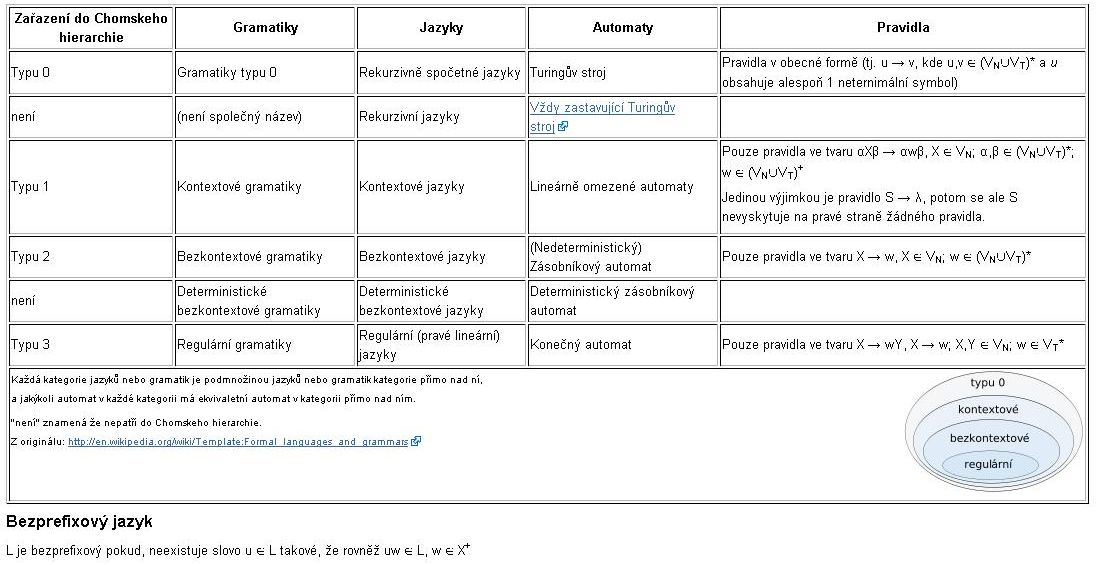
\includegraphics[scale=1.7]{informatika/teoreticka_informatika/obrazky/chomski.png}
  \end{center}
\end{figure}
\end{e}

\begin{e}{Pozn�mka}{0}{0}
S $\c{L}1 \supset \c{L}2$ nast�v� probl�m, proto�e bezkontextov� gramatiky umo��uj� pravidla tvaru $X\to\lambda$. �e�en�m je p�evod na \emph{nevypou�t�j�c� bezkontextov� gramatiky} - takov� bezkontextov� gramatiky, kter� nemaj� pravidla typu $X\to\lambda$.
\end{e}

\begin{e}{V�ta}{0}{o nevypou�t�j�c�ch bezkontextov�ch gramatik�ch}
Ke ka�d� bezkontextov� $G$ existuje nevypou�t�j�c� bezkontextov� $G_0$ tak, �e $$L(G_0)=L(G)\setminus\{\lambda\}$$ Je-li $\lambda\in L(G)$, pak $\exists G_1$, t.�. $L(G_1)=L(G)$ a jedin� pravidlo v $G_1$ s $\lambda$ na prav� stran� je $S\to\lambda$ a $S$ nen� v $G_1$ na prav� stran� ��dn�ho pravidla.
\end{e}

\begin{e}{Pozn�mka}{0}{Line�rn� gramatiky}
Pro ka�dou gramatiku typu G3 lze sestrojit kone�n� automat, kter� p�ij�m� pr�v� jazyk j� generovan�, stejn� tak pro ka�d� kone�n� automat lze sestrojit gramatiku G3. Lev� line�rn� gramatiky tak� generuj� regul�rn� jazyky, d�ky uzav�enosti na reverzi. \emph{Line�rn� gramatiky}, s pravidly typu $X\to uYv,X\to w$, kde $X,Y\in V_N, u,v,w\in V_T^{\ast}$, generuj� \emph{line�rn� jazyky} - siln�j�� ne� regul�rn� jazyky.
\end{e}

\begin{e}{Definice}{0}{Separovan� a nevypou�t�j�c� gramatika}
\emph{Separovan� gramatika} je gramatika (obecn� libovoln� t��dy), obsahuj�c� pouze pravidla tvaru $\alpha\to\beta$, kde bu� $\alpha,\beta\in V_N^+$, nebo $\alpha\in V_N$ a $\beta\in V_T\cup\{\lambda\}$. \emph{Nevypou�t�j�c� (monot�nn�) gramatika} (tak� se neomezuje na konkr�tn� t��du) je takov�, �e pro ka�d� pravidlo $u\to v$ plat� $|u|\leq|v|$.
\end{e}

\begin{e}{Pozn�mka}{0}{Kontextov� gramatiky}
Ke ka�d� kontextov� gramatice lze sestrojit ekvivalentn� separovanou. Ke ka�d� monot�nn� gramatice lze nal�zt ekvivalentn� kontextovou.
\end{e}


\subsubsection*{Determinismus a nedeterminismus}

\begin{e}{Definice}{0}{Nedeterministick� kone�n� automat}
\emph{Nedeterministick� kone�n� automat} je p�tice $(Q,X,\delta,S,F)$, kde $Q$ je mn. stav�, $X$ abeceda, $F$ mn. konc. stav�, $S$ mno�ina po��te�n�ch stav� a $\delta:Q\times X\to \c{P}(Q)$ je p�echodov� funkce. Slovo $w$ je takov�m automatem p�ij�m�no, pokud existuje posloupnost stav� $\{q_i\}_{i=1}^n$ tak, �e $q_1\in S$, $q_{i+1}\in\delta(q_i,x_i)$, $q_{n+1}\in F$.
\end{e}

\begin{e}{Pozn�mka}{0}{0}
Pro ka�d� nedeterministick� kone�n� automat $A$ lze sestrojit deterministick� kon. automat $B$ tak, �e jimi p�ij�man� jazyky jsou ekvivalentn� (m��e to znamenat exponenci�ln� n�r�st po�tu stav�).
\end{e}


\begin{e}{Definice}{0}{Deterministick� z�sobn�kov� automat}
\emph{Deterministick� z�sobn�kov� automat} je $M=(Q,X,Y,\delta,q_0,Z_0,F)$ takov�, �e $\forall p\in Q, \forall a\in (X\cup\{\lambda\}), \forall Z\in Y$ plat� $|\delta(p,a,Z)|\leq 1\footnote{definuje ze v kazdem kroku si nemuzeme vybirat}$ a nav�c pokud pro n�jak� $p, Z$ je $\delta(p,\lambda,Z)\neq\emptyset$, pak $\forall a\in X$ je $\delta(p,a,Z)=\emptyset\footnote{definuje ukon�en� vypoctu}$. 
\end{e}

\begin{e}{Pozn�mka}{0}{0}
Deterministick� z�sobn�kov� automat je \uv{slab��} ne� nedeterministick�, rozpozn�v� \emph{deterministick� bezkontextov� jazyky} koncov�m stavem a \emph{bezprefixov� bezkontextov� jazyky} pr�zdn�m z�sobn�kem (takov� jazyky, kde $u\in L(M)\implies \forall w\in X^{\ast}: uw\notin L(M)$) - kdy� se poprv� z�sobn�k automatu vypr�zdn�, v�po�et ur�it� kon��. 

Bezprefixov� bezkontextov� jazyky jsou v�dy deterministick�, opa�n� to neplat�. Deterministick� bezkontextov� jazyk lze na bezprefixov� p�ev�st z�et�zen�m s dal��m symbolem, kter� nen� v p�vodn� abeced�. 

Regul�rn� jazyky a bezprefixov� bezkontextov� jazyky jsou neporovnateln� mno�iny.
\end{e}

\begin{e}{Definice}{0}{Nedeterministick� Turing�v stroj}
\emph{Nedet. Turing�v stroj} je p�tice $T=(Q,X,\delta,q_0,F)$, kde oproti deterministick�m je $\delta:(Q\setminus F)\times X \to \c{P}(Q\times X\times \{-1,0,1\})$. P�ij�m� slovo $w$, pokud existuje n�jak� v�po�et $q_{0}w\vdash^{\ast} upv$ tak, �e $p\in F$.
\end{e}

\begin{e}{Pozn�mka}{0}{0}
Nedeterministick� Turingovy stroje p�ij�maj� pr�v� rekurzivn� spo�etn� jazyky, tj. nejsou siln�j�� ne� deterministick�. V�po�ty nedet. stroje lze toti� d�ky nekone�nosti p�sky simulovat deterministick�m (nap�. prohled�v�n�m do ���ky).
\end{e}

\begin{e}{Definice}{0}{Line�rn� omezen� automat}
\emph{Line�rn� omezen� automat} je nedeterministick� Turing�v stroj s omezenou p�skou (nap�. symboly $l$ a $r$, kter� nelze p�epsat ani se dostat mimo jejich rozmez�). Slovo je p�ij�m�no, pokud $q_{0}lwr \vdash^{\ast} upv$, kde $p\in F$. Prostor v�po�tu je omezen d�lkou vstupn�ho slova. Line�rn� omezen� automaty p�ij�maj� pr�v� kontextov� jazyky.
\end{e}


\begin{e}{Pozn�mka}{0}{Rozhodnutelnost}
Turing�v stroj m��e nep�ijmout slovo bu� skon�en�m v�po�tu v nekoncov�m stavu, nebo pokud v�po�et nikdy neskon��. Turing�v stroj \emph{rozhoduje jazyk} $L$, kdy� p�ij�m� pr�v� slova tohoto jazyka a pro libovoln� slovo je jeho v�po�et kone�n�. Takov� jazyky se naz�vaj� \emph{rekurzivn�}.

Probl�m zastaven� v�po�tu Turingova stroje je algoritmicky nerozhodnuteln� (kv�li mo�nosti jeho simulace jin�m Turingov�m strojem). Pro bezkontextov� jazyky je algoritmicky rozhodnuteln�, zda dan� slovo pat�� do jazyka. Pro bezkontextovou gramatiku nelze algoritmicky rozhodnout, zda $L(G)=X^{\ast}$. Pro dv� kontextov� gramatiky je nerozhodnuteln�, zda jejich jazyky maj� nepr�zdn� pr�nik.
\end{e}

\begin{reportN}{Hnetynka}
napisal som hierachiu, pravidla gramatik, ake automaty rozpoznavaju jednotlive gramatiky, pre reg gram veticky o KA a reg jazykoch. Pytal sa ma ako jednotlive automaty pracuju, zadal par jednoduchych prikladov a chcel zdovodnenie do akych tried patri -nakreslit/opisat slovami KA, gramatiky, ZA + dokaz pomocou pumping lemma. Pytal sa, do akej triedy by som zaradil rozpoznavanie prg jazykov, napr Java. Povedal som kontextove, ale zdovodnit som to velmi nevedel. Potvrdil ze su to kontextove + ze prave kvoli dobrym znalostam sa pouzivaju bezkontextove v kombinacii s analyzou kontextu (kedze na poradi jednotlivych riadkov zalezi) (znamka 1-2, ze zalezi na druhej inf otazke)
\end{reportN}

\begin{reportN}{Bulej}
napisal som gramatiky, odpovedajuce automaty, vysvetlil inkluzie a to bohato stacilo
\end{reportN}
\begin{reportN}{Bednarek}
M�l jsem definice hierarchie a srovn�n� s p��slu�n�mi automaty, n�stin (opravdu lehce) inkluz� mezi t��dami jazyk�, Greibachov� a Chomsk�ho n.f. plus n�jak� p��klady jazyk�, kter� dokazuj� ostrou inkluzi, ale bez p�esn�j��ch d�kaz� (kouzeln� v�ta: "to se uk�e p�es pumping lemma" ;-) ) Ptal se m� na srovn�n� deterministick�ch a nedeterministick�ch verz� jednotliv�ch druh� automat�, co� jsem v�d�l.
Informatika za jedna.
\end{reportN}
\begin{reportN}{Kucera}
Toto se obeslo bez problemu, stacilo to definovat, a rict ktere automaty prijimaij ktere jazyky, umet je definovat. Vety kolem moc zajem nevzbudily ( Nerudovka, pump. lemma):-) 
\end{reportN}
\begin{reportN}{Fiala}
Napsal sem t��dy automat�, gramatik, determinismus/nedeterminismus a pak je�t� rozhodnutelnost. P�i proch�zen� sem dost�val dopl�uj�c� ot�zky typu : "Jak n�jak l�p omezit odhad o n�rustu po�tu stavu p�i p�evodu NKA do KA" (z�le�� na po�tu po��te�n�ch stav� a na po�tu "stejnejch" p�echod� z jednotliv�ch stav�.), U rozhodnutelnosti n�znak d�kazu halting problem a dal��.
\end{reportN}
\begin{reportN}{Bedn�rek}
Tak jsem napsal automat a gramatiku ke ka�d� t��d� jazyk�, determ./nedeterm. verze a jak je to kde s jejich silou. Drobn� chyby v definic�ch nevadily, kdy� byly po upozorn�n� opraveny. U RJ se zeptal je�t� na reg. v�razy a pak taky pro� �e se rekurzivn� spo�etn� jazyky jmenuj� jak se jmenuj� (kde je ta rekurze), co� jsem nev�d�l a byl pou�en.
\end{reportN}
\begin{reportN}{IOI 10.2.2011} 
a) Popi�te jednotliv� t��dy jazyk� a jejich vztahy definujte t��dy pomoc� odpovidajicich gramatik. Napi�te p�iklady gramatik pro jednotliv� t��dy.
\\b) Popi�te automaty, ktere tyto t��dy jazyk� rozpozn�vaj� i s ohledem na jejich (ne)determinsti�nost.
\end{reportN}
\begin{reportN}{IOI 21. 6. 2011} 4.1 Popi�te Chomsk�ho hierarchii t��d jazyk�, jak se naz�vaj� jazyky v ka�d� t��d�, jak� typ gramatiky je generuje a jak� typ automatu je p�ij�m�.\\
4.2 Uve�te p��klad neregul�rn�ho jazyka a uka�te, �e nen� regul�rn�.\\
\textbf{4.3 Existuje uz�v�rov� vlastnost, na kterou nejsou uzav�en� jazyky typu 0?} TODO
\end{reportN} 
\begin{reportN}{IP 21. 6. 2011} 
Uka�te, �e n�sleduj�c� gramatika G je v�cezna�n� $S \rightarrow if\, then\, S\, else\, S\, | if\, then\, S\, | \lambda$\\
Vytvo�te gramatiku G', kter� nebude v�cezna�n�, a bude platit $L(G) = L(G')$.\\
Existuje obecn� k libovoln� bezkontextov� gramatice G jednozna�n� gramatika G' takov�, �e $L(G) = L(G')$?
\end{reportN} 



\end{document}
